%%%%%%%%%%%%%%%%%%%%%%%%%%%%%%%%%%%%%%%%%%%%%%%%%%%%%%%%%%%%%%%%%%%%%
%
% CSCI 1430 Written Question Template
%
% This is a LaTeX document. LaTeX is a markup language for producing documents. 
% You will fill out this document, compile it into a PDF document, then upload the PDF to Gradescope. 
%
% To compile into a PDF on department machines:
% > pdflatex thisfile.tex
%
% If you do not have LaTeX, your options are:
% - Personal laptops (all common OS): http://www.latex-project.org/get/ 
% + VSCode extension: https://marketplace.visualstudio.com/items?itemName=James-Yu.latex-workshop
% - Online Tool: https://www.overleaf.com/ - most LaTeX packages are pre-installed here (e.g., \usepackage{}).
%
% If you need help with LaTeX, please come to office hours.
% Or, there is plenty of help online:
% https://en.wikibooks.org/wiki/LaTeX
%
% Good luck!
% The CSCI1430 staff
%
%%%%%%%%%%%%%%%%%%%%%%%%%%%%%%%%%%%%%%%%%%%%%%%%%%%%%%%%%%%%%%%%%%%%%

\documentclass{csci1430}

\begin{document}
\title{Homework 3 Written Questions}
\maketitle
\thispagestyle{fancy}

\writeinstructions

\section*{This Homework}
\begin{itemize}
  \item 6 questions \textbf{[10 + 8 + 4 + 10 + 3 + 12 = 47 points + 2 bonus points]}.
  \item Include code, images, and equations where appropriate.
\end{itemize}

%%%%%%%%%%%%%%%%%%%%%%%%%%%%%%%%%%%%%%%%
\pagebreak

\begin{question}[points=10,drawbox=false]
Suppose we have a two quadrilaterals $\mathbf{abcd}$ and $\mathbf{a'b'c'd'}$:

\begin{minipage}[c]{0.49\textwidth}
    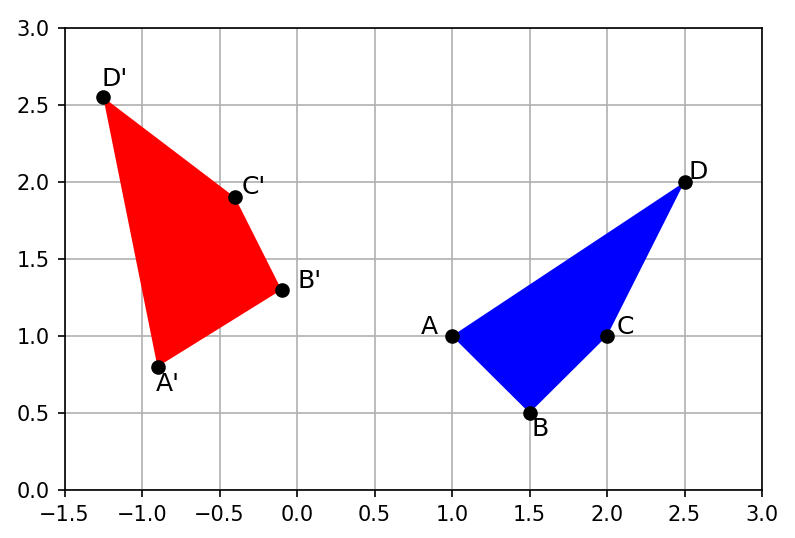
\includegraphics[width=\textwidth]{images/quads_lstsq.png}
\end{minipage}
\begin{minipage}[c]{0.49\textwidth}
    \begin{equation*}
    \begin{split}
    \mathbf{a}&=(1, 1)\\
    \mathbf{b}&=(1.5, 0.5)\\
    \mathbf{c}&=(2, 1)\\
    \mathbf{d}&=(2.5, 2)
    \end{split}
    \quad\quad\quad
    \begin{split}
    \mathbf{a'}&=(-0.9, 0.8)\\
    \mathbf{b'}&=(-0.1, 1.3)\\
    \mathbf{c'}&=(-0.4, 1.9)\\
    \mathbf{d'}&=(-1.25, 2.55)
    \end{split}
    \end{equation*}
\end{minipage}

They look like they are related by a rotation and a non-uniform scale transformation. So, let's assume that each point in $\mathbf{abcd}$ could be mapped to its corresponding point in $\mathbf{a'b'c'd'}$ by a $2\times2$ transformation matrix $\mathbf{M}$, as these can represent non-linear scaling and rotation.

e.g., if 
$\mathbf{p} = \begin{bmatrix} x \\ y \end{bmatrix}$, 
$\mathbf{p'} = \begin{bmatrix} x' \\ y' \end{bmatrix}$,
and 
$\mathbf{M} = \begin{bmatrix} m_{1,1} & m_{1,2} \\ m_{2,1} & m_{2,2} \end{bmatrix}$,

then $\begin{bmatrix} m_{1,1} & m_{1,2} \\ m_{2,1} & m_{2,2} \end{bmatrix} \begin{bmatrix} x \\ y \end{bmatrix} = \begin{bmatrix} x' \\ y'  \end{bmatrix}$

\end{question}

\begin{subquestion}[points=1]
Rewrite the equation $\mathbf{M}\mathbf{p} = \mathbf{p'}$ into a pair of linear equations by expanding the matrix multiplication symbolically.
\end{subquestion}

\begin{answer}
TODO: Replace each of the `$\_\_$' below with $x, y, x', y',$ or $0$.
\begin{align*}
\begin{cases}
    \_\_m_{1,1} + \_\_m_{1,2} + \_\_m_{2,1} + \_\_m_{2,2} = \_\_
    \\\_\_m_{1,1} + \_\_m_{1,2} + \_\_m_{2,1} + \_\_m_{2,2} = \_\_
\end{cases}
\end{align*}
\end{answer}

\clearpage
\begin{subquestion}[points=2,drawbox=false]
We would like to estimate $\mathbf{M}$ using least squares linear regression. For this, we form a system of linear equations, typically written in the form $\mathbf{Ax}=\mathbf{b}$, where $\mathbf{x}$ contains the parameters of $\mathbf{M}$, matrix $\mathbf{A}$ contains the coordinates of $\mathbf{p}$ and column vector $\mathbf{b}$ contains the corresponding coordinates of $\mathbf{p'}$.
\begin{align*}
    \mathbf{Ax}=\mathbf{b} \hspace{0.4cm}\text{where}\hspace{0.4cm} \mathbf{A} \times \begin{bmatrix} m_{1,1} \\ m_{1,2} \\ m_{2,1} \\ m_{2,2} \\ \end{bmatrix} = \mathbf{b}
\end{align*}
%
As $\mathbf{M}$ has four parameters, we need four equations to \emph{determine} an $\mathbf{M}$. As each point pair provides two equations, that $\mathbf{M}$ will exactly transform those two points $\mathbf{p}$ onto their pairs $\mathbf{p'}$. But, as our quadrilaterals have four points, we could create eight such equations to estimate $\mathbf{M}$---$\mathbf{M}$ is now said to be \emph{overdetermined}. If all point pairs \emph{do not} exactly transform by some $\mathbf{M}$, then using an overdetermined system will find an $\mathbf{M}$ that minimize the distance (or residual error) between all estimated values for $\mathbf{p'}$ and the real values for $\mathbf{p'}$, i.e., that minimize the Euclidean norm (or 2-norm) $||\mathbf{A}\mathbf{x} - \mathbf{b}||_2$.

\emph{Note:} As systems of linear equations are typically written in the form $\mathbf{Ax}=\mathbf{b}$, we've overloaded the symbol $\mathbf{b}$ here to keep this familiarity. So, be careful---$\mathbf{b}$ is the vector of target $x',y'$ values across all equations, and not the point in the quadrilateral.
\end{subquestion}

\begin{orangebox}
Declare $\mathbf{A}$ and $\mathbf{b}$ for all four point pairs.\\

Replace each `$\_\_$' below with a $0$ or a coordinate value from the quadrilaterals.
\end{orangebox}

\begin{answer}
\begin{align*}
    \begin{bmatrix} 
    \_\_ & \_\_ & \_\_ & \_\_ \\ 
    \_\_ & \_\_ & \_\_ & \_\_ \\ 
    \_\_ & \_\_ & \_\_ & \_\_ \\ 
    \_\_ & \_\_ & \_\_ & \_\_ \\ 
    \_\_ & \_\_ & \_\_ & \_\_ \\ 
    \_\_ & \_\_ & \_\_ & \_\_ \\ 
    \_\_ & \_\_ & \_\_ & \_\_ \\ 
    \_\_ & \_\_ & \_\_ & \_\_
    \end{bmatrix} 
    \times \begin{bmatrix} m_{1,1} \\ m_{1,2} \\ m_{2,1} \\ m_{2,2} \\ \end{bmatrix} 
    = \begin{bmatrix} 
    \_\_ \\ 
    \_\_ \\ 
    \_\_ \\ 
    \_\_ \\ 
    \_\_ \\ 
    \_\_ \\ 
    \_\_ \\ 
    \_\_ 
    \end{bmatrix}
\end{align*}
\end{answer}


\clearpage
\begin{subquestion}[points=3,drawbox=false]
If we use four equations, then $\mathbf{A}$ is square and can be easily inverted to solve for $\mathbf{x}$ by left multiplying the inverse by both sides:
%
\begin{equation}
\mathbf{A}^{-1} \mathbf{A}\mathbf{x} = \mathbf{A}^{-1} \mathbf{b} \hspace{0.5cm}\text{so}\hspace{0.5cm} \mathbf{x} = \mathbf{A}^{-1} \mathbf{b}.
\end{equation}
%
If we use more than four equations, then $\mathbf{A}$ is non-square. In this situation, we can use the pseudoinverse of $\mathbf{A}$, written as $\mathbf{A}^+$.
\begin{equation}
\mathbf{A}^+ \mathbf{A}\mathbf{x} = \mathbf{A}^+ \mathbf{b}
\hspace{0.5cm}\text{so}\hspace{0.5cm} \mathbf{x} = \mathbf{A}^+ \mathbf{b}.
\end{equation}
    
As long as $\mathbf{A}$ has a pseudoinverse, this solution minimizes $||\mathbf{A}\mathbf{x} - \mathbf{b}||_2$.\\ 
This is the closed-form least squares solution, where $\mathbf{x} = (\mathbf{A}^\top \mathbf{A})^{-1}\mathbf{A}^\top\mathbf{b}$ and where $\mathbf{A}^+ = (\mathbf{A}^\top \mathbf{A})^{-1}\mathbf{A}^\top$.
    
We can compute the pseudoinverse from the singular value decomposition. In python, \texttt{numpy.linalg.lstsq()} will handle this for us, including solving large systems. \texttt{lstsq()} takes as input $\mathbf{A}$ and $\mathbf{b}$, and returns a solution for $\mathbf{x}$ along with the residual error. Plug your $\mathbf{A}$,$\mathbf{b}$ values into that function and write the numeric values of the estimated $\mathbf{M}$ matrix below along with the numeric value of the residual error.
    
\textit{Note:} We provide a Python script \texttt{transformation\_viz.py} for you to estimate and visualize the transformation. Within function \texttt{estimate\_transform()}, declare matrix $\mathbf{A}$ and vector $\mathbf{b}$ and create a function call to \texttt{lstsq()} to see how the quadrilaterals match up!
\end{subquestion}

\begin{orangebox}
State your $\mathbf{M}$ by replacing each of the `$\_\_$' below, and state the residual error.
\end{orangebox}

\begin{answer}
\begin{align*}
    \textbf{M} = \begin{bmatrix} m_{1,1} & m_{1,2} \\ m_{2,1} & m_{2,2} \end{bmatrix} = \begin{bmatrix} \_\_ & \_\_ \\ \_\_ & \_\_ \end{bmatrix}
\end{align*}

Residual error: xxx
\end{answer}

\pagebreak
\begin{subquestion}[points=4,drawbox=false]
If the residual is zero (or zero to machine numerical precision), then we can confirm our initial assumption that the transformation is a rotation and a scale. If it is not, then we need a transformation with more degrees of freedom to reduce the residual error.
\end{subquestion}

\begin{orangebox}
Determine what kind of transformation it is by forming a system of linear equations and estimating an $\mathbf{M}$ that produces zero residual error (to machine numerical precision).\\

Use your implementation in \texttt{transformation\_viz.py} to help.
Write out your system's $\mathbf{A}$, $\mathbf{x}$, and $\mathbf{b}$ matrices, state $\mathbf{M}$ and the residual error, and state which kind of transformation it is.
\end{orangebox}
    
\begin{answer}[height=30]
% Copy the templates from above. As your M can vary, we don't know ahead of time which solution you will use, so we cannot provide the templates.
\end{answer}



%%%%%%%%%%%%%%%%%%%%%%%%%%%%%%%%%%%
% Please leave the pagebreak
\pagebreak
\begin{question}[points=8,drawbox=false]
In lecture, we've learned that cameras can be represented by intrinsic and extrinsic matrices. These matrices can be used to calculate the projections of points within a 3D world onto 2D image planes. For this, we use \emph{homogeneous coordinates}. The final $3\times4$ matrix is known as the \emph{camera matrix}.

Recall that the transformation can be represented by the following expression:
\begin{align*}
    \begin{bmatrix} 
    f_x & s & $0$ \\ 
    $0$ & f_y & $0$ \\ 
    $0$ & $0$ & $1$ \end{bmatrix} \times
    \begin{bmatrix} 
    r_{11} & r_{12} & r_{13} & t_x \\ 
    r_{21} & r_{22} & r_{23} & t_y \\  
    r_{31} & r_{32} & r_{33} & t_z
    \end{bmatrix} \times 
    \begin{bmatrix} 
    x \\ 
    y \\ 
    z \\ 
    $1$ \end{bmatrix}
    = w
    \begin{bmatrix}  u \\ v \\ $1$ \end{bmatrix}
\end{align*}
where $f$ is the focal length, $\mathbf{R}$ is the rotation matrix, $\mathbf{t}$ is the translation vector,  $w$ is some weighing/scaling factor, and $(u, v)$ is the position that the point in the real world $(x, y, z)$ projects to on the 2D plane.

For each following question, you are given the camera specifications and a sample 3D point from the real world. Fill in the camera's intrinsic $\mathbf{K}$ and extrinsic $\mathbf{[Rt]}$ matrices; then, perform the multiplications and perspective division (unhomogenize) to find the 2D coordinate of the projected point.
\end{question}

\begin{subsubquestion}[points=1]
A camera with a focal length of 1 in both the $x$ and $y$ directions, a translation of 5 along the $x$-axis, and no skew or rotation.
\end{subsubquestion}

\begin{answer}
TODO: Fill in the \_\_ entries.
\begin{align*}
    & \hspace{1.3cm} \mathbf{K} \hspace{0.8cm} \times \hspace{1cm} [\mathbf{R} \mathbf{t}] \hspace{0.9cm} \times \; 
    \begin{bmatrix} 
        x  \\ 
        y  \\ 
        z  \\
        1
    \end{bmatrix} \\
    &= \begin{bmatrix} 
    \_\_ & \_\_ & $0$    \\  % <----- TODO: replace \_\_ %
    $0$ & \_\_ & $0$     \\  % <----- TODO: replace \_\_ %
    $0$ & $0$ & $1$ 
    \end{bmatrix} 
    \times
    \begin{bmatrix} 
    \_\_ & \_\_ & \_\_ & \_\_  \\ % <----- TODO: replace \_\_ %
    \_\_ & \_\_ & \_\_ & \_\_  \\ % <----- TODO: replace \_\_ %
    \_\_ & \_\_ & \_\_ & \_\_     % <----- TODO: replace \_\_ %
    \end{bmatrix} \times
    \begin{bmatrix} 
    $30$    \\ 
    $-20$   \\ 
    $10$    \\ 
    $1$ \end{bmatrix} \\
    &= \qquad \qquad \qquad \begin{bmatrix} 
    \_\_    \\   % <----- TODO: replace \_\_ %
    \_\_    \\   % <----- TODO: replace \_\_ %
    \_\_         % <----- TODO: replace \_\_ %
    \end{bmatrix} \\
    &= \qquad \quad \quad 
    \_\_         % <----- TODO: replace \_\_ %
    \times 
    \begin{bmatrix}  
    \_\_    \\   % <----- TODO: replace \_\_ %
    \_\_    \\   % <----- TODO: replace \_\_ %
    $1$ 
    \end{bmatrix}
\end{align*}
\end{answer}


\pagebreak
\begin{subsubquestion}[points=1]
A camera with focal length of $2$ in both the $x$ and $y$ directions, a translation of $5$ along the $x$-axis, and no skew or rotation.
\end{subsubquestion}

\begin{answer}
\begin{align*}
    &= \begin{bmatrix} 
    \_\_ & \_\_ & $0$    \\  % <----- TODO: replace \_\_ %
    $0$ & \_\_ & $0$     \\  % <----- TODO: replace \_\_ %
    $0$ & $0$ & $1$ 
    \end{bmatrix} 
    \times
    \begin{bmatrix} 
    \_\_ & \_\_ & \_\_ & \_\_  \\ % <----- TODO: replace \_\_ %
    \_\_ & \_\_ & \_\_ & \_\_  \\ % <----- TODO: replace \_\_ %
    \_\_ & \_\_ & \_\_ & \_\_     % <----- TODO: replace \_\_ %
    \end{bmatrix} \times
    \begin{bmatrix} 
    $30$    \\ 
    $-20$   \\ 
    $10$    \\ 
    $1$ \end{bmatrix} \\
    &= \qquad \qquad \qquad \begin{bmatrix} 
    \_\_    \\   % <----- TODO: replace \_\_ %
    \_\_    \\   % <----- TODO: replace \_\_ %
    \_\_         % <----- TODO: replace \_\_ %
    \end{bmatrix} \\
    &= \qquad \quad \quad 
    \_\_         % <----- TODO: replace \_\_ %
    \times 
    \begin{bmatrix}  
    \_\_    \\   % <----- TODO: replace \_\_ %
    \_\_    \\   % <----- TODO: replace \_\_ %
    $1$ 
    \end{bmatrix}
\end{align*}
\end{answer}


\begin{subquestion}[points=2]
Compare the two image coordinates you've calculated in parts a and b. Explain how each parameter affects the final image coordinate. \textbf{[2-3 sentences]}
\end{subquestion}

\begin{answer}[height=12]
\end{answer}


%%%%%%%%%%%%%%%%%%%%%%%%%%%%%%%%%%%
\pagebreak

\begin{subquestion}[points=4,drawbox=false]
In the questions folder, we provide stencil code for a camera simulation in \texttt{camera\_simulation.py}. Given a camera matrix, the simulator visualizes an image that a camera would produce. 
\end{subquestion}

\begin{orangebox}
Please implement \texttt{calculate\_camera\_matrix()} by calculating the camera matrix using the parameters given in the code. When successful, you will see a bunny rendered as dots (as below). Paste your code for this function and attach a screenshot of the working demo once you finish. Play around with the sliders to see how different parameters affect the projection!
\end{orangebox}

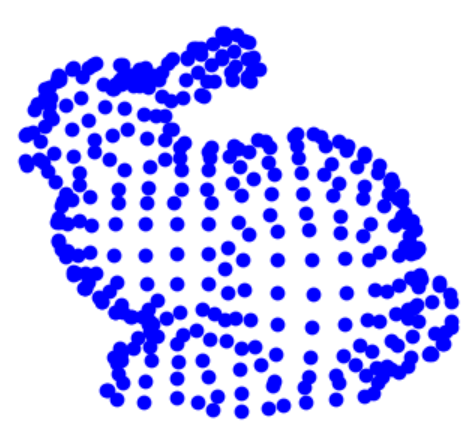
\includegraphics[width=0.5\linewidth]{images/bunny.png}

\begin{answer}

\includegraphics[width=0.7\textwidth,keepaspectratio]{images/TODO_demo_screenshot.png}
\end{answer}

\begin{answer}[height=46]
\begin{python}
def calculate_camera_matrix(tx, ty, tz, alpha, beta, gamma, fx, fy, skew, u, v):
    ########################
    # TODO: Your calculate_camera_matrix() code here #
    # Hint: Calculate the rotation matrices for the x, y, and z axes separately.
    # Then multiply them to get the rotational part of the extrinsic matrix.
    ########################
    
    return (initial_camera_matrix_to_replace, 
    initial_intrinsic_matrix_to_replace, 
    initial_extrinsic_matrix_to_replace)
\end{python}
\end{answer}

\pagebreak
\begin{answer}[height=46]
\begin{python}
################################################
# YOU MAY USE THIS ADDITIONAL PAGE

# WARNING: IF YOU DON'T END UP USING THIS PAGE
# KEEP THESE COMMENTS TO MAINTAIN PAGE ALIGNMENT
################################################
\end{python}
\end{answer}
    


%%%%%%%%%%%%%%%%%%%%%%%%%%%%%%%%%%%
\pagebreak
\begin{question}[points=4,drawbox=false]
\end{question}

\begin{subquestion}[points=2]
Given a stereo pair of cameras, briefly describe triangulation. Describe the inputs and outputs of the process. You may wish to use a diagram. \textbf{[3--4 sentences]}
\end{subquestion}

\begin{answer}[height=30]
\end{answer}

\pagebreak
\begin{subquestion}[points=2]
Why is it not possible to find an absolute depth for each point when we don't have calibration information for our cameras? Note that absolute depth refers to depth with respect to the camera as opposed to relative depth, which is with respect to another object in the scene. \textbf{[3 - 4 sentences]}
\end{subquestion}

\begin{answer}[height=10]
\end{answer}


%%%%%%%%%%%%%%%%%%%%%%%%%%%%%%%%%%%
\pagebreak

\begin{question}[points=10,drawbox=false]
Given the algorithms that we've learned in computer vision, we know that whether we can find/calculate the essential matrix, the fundamental matrix, or both depends on the setup of the cameras and images. You are given three datasets of an object of unknown geometry:

\begin{enumerate}[(i)]
\item A video circling the object;
\item A stereo pair of calibrated cameras capturing two images of the object; and
\item Two images of the same object on the internet (e.g. Colosseum) at different camera poses but with unknown intrinsics.
\end{enumerate}
\end{question}

\begin{orangebox}[points=3]
For each of the above setups, what calculations can we perform? Provide brief explanations to support your choice(s). \textbf{[1 - 2 sentences]}
\end{orangebox}
\begin{enumerate}[(i)]
\item Setup 1
\begin{answerlist}
    \item Essential Matrix
    \item Fundamental Matrix
    \item Both
\end{answerlist}

\item Setup 2
\begin{answerlist}
    \item Essential Matrix
    \item Fundamental Matrix
    \item Both
\end{answerlist}

\item Setup 3
\begin{answerlist}
    \item Essential Matrix
    \item Fundamental Matrix
    \item Both
\end{answerlist}

\end{enumerate}

\begin{subquestion}[points=3]
State an advantage and disadvantage of using each setup for depth reconstruction. \textbf{[2 - 3 sentences]}
\end{subquestion}

\begin{enumerate}[(i)]
    \item Setup 1
    \begin{tcolorbox}[colback=white!5!white,colframe=green!75!black]
        \setbox0=\hbox{\parbox[t]{\textwidth}{
            %%%%%%% ANSWER STARTS HERE %%%%%%%%%%%%%%%%%%%%%%%%%%%%

            TODO: Your answer to (b) (i) here.

            %%%%%%% ANSWER ENDS HERE %%%%%%%%%%%%%%%%%%%%%%%%%%%%%%
            }}
        \clipbox{0pt \dimexpr\dp0-7\baselineskip\relax{} 0in 0pt}{\copy0}
    \end{tcolorbox}
    \item Setup 2
    \begin{tcolorbox}[colback=white!5!white,colframe=green!75!black]
        \setbox0=\hbox{\parbox[t]{\textwidth}{
            %%%%%%% ANSWER STARTS HERE %%%%%%%%%%%%%%%%%%%%%%%%%%%%

            TODO: Your answer to (b) (ii) here.

            %%%%%%% ANSWER ENDS HERE %%%%%%%%%%%%%%%%%%%%%%%%%%%%%%
            }}
        \clipbox{0pt \dimexpr\dp0-7\baselineskip\relax{} 0in 0pt}{\copy0}
    \end{tcolorbox}
    \item Setup 3
    \begin{tcolorbox}[colback=white!5!white,colframe=green!75!black]
        \setbox0=\hbox{\parbox[t]{\textwidth}{
            %%%%%%% ANSWER STARTS HERE %%%%%%%%%%%%%%%%%%%%%%%%%%%%

            TODO: Your answer to (b) (iii) here.

            %%%%%%% ANSWER ENDS HERE %%%%%%%%%%%%%%%%%%%%%%%%%%%%%%
            }}
        \clipbox{0pt \dimexpr\dp0-7\baselineskip\relax{} 0in 0pt}{\copy0}
    \end{tcolorbox}
\end{enumerate}

% \item \textbf{[3 $\times$ 1 points]}
% \begin{tcolorbox}[colback=orange!5!white,colframe=orange!75!black]
% Name an application scenario for each of the different setups \textbf{[1 - 2 sentences]}
% \end{tcolorbox}
% \begin{enumerate}[(i)]
%     \item Setup 1
%     \begin{tcolorbox}[colback=white!5!white,colframe=green!75!black]
%         \setbox0=\hbox{\parbox[t]{\textwidth}{
%             %%%%%%% ANSWER STARTS HERE %%%%%%%%%%%%%%%%%%%%%%%%%%%%

%             TODO: Your answer to (c) (i) here.

%             %%%%%%% ANSWER ENDS HERE %%%%%%%%%%%%%%%%%%%%%%%%%%%%%%
%             }}
%         \clipbox{0pt \dimexpr\dp0-10\baselineskip\relax{} 0in 0pt}{\copy0}
%     \end{tcolorbox}
%     \item Setup 2
%     \begin{tcolorbox}[colback=white!5!white,colframe=green!75!black]
%         \setbox0=\hbox{\parbox[t]{\textwidth}{
%             %%%%%%% ANSWER STARTS HERE %%%%%%%%%%%%%%%%%%%%%%%%%%%%

%             TODO: Your answer to (c) (ii) here.

%             %%%%%%% ANSWER ENDS HERE %%%%%%%%%%%%%%%%%%%%%%%%%%%%%%
%             }}
%         \clipbox{0pt \dimexpr\dp0-10\baselineskip\relax{} 0in 0pt}{\copy0}
%     \end{tcolorbox}
%     \item Setup 3
%     \begin{tcolorbox}[colback=white!5!white,colframe=green!75!black]
%         \setbox0=\hbox{\parbox[t]{\textwidth}{
%             %%%%%%% ANSWER STARTS HERE %%%%%%%%%%%%%%%%%%%%%%%%%%%%

%             TODO: Your answer to (c) (iii) here.

%             %%%%%%% ANSWER ENDS HERE %%%%%%%%%%%%%%%%%%%%%%%%%%%%%%
%             }}
%         \clipbox{0pt \dimexpr\dp0-10\baselineskip\relax{} 0in 0pt}{\copy0}
%     \end{tcolorbox}
% \end{enumerate}

\begin{subquestion}[points=4]
The differences between the collection methods for these three datasets are crucial in terms of what calculations are possible - and therein which applications they are most useful in.
\end{subquestion}

\begin{orangebox} 
From a non-technical standpoint, can you think of a scenario why you may prefer one of these data collection setups to another? Why is it important to know what data collection methods have been used to build a particular dataset? \textbf{[5-7 sentences]}
\end{orangebox}

\begin{answer}[height=20]
\end{answer}


%%%%%%%%%%%%%%%%%%%%%%%%%%%%%%%%%%%
% Please leave the pagebreak
\pagebreak 
\paragraph{Q5:} \textbf{[3 points]} In two-view camera geometry, what do the following epipolar lines say about the cameras' relative positions? \textbf{[1 - 2 sentences each]}

\textit{Tip:} The Spring '22 course staff created an \href{https://browncsci1430.github.io/resources/stereo_camera_visualization_demo/}{interactive demo} to explore the different scenarios and get a better feel for epipolar geometry.

\begin{enumerate}[(a)]
\item Please draw or describe the relative positions of the two camera planes. Check slides from the lecture on stereo geometry for details of carera planes.
\textbf{[1 point]} 
\begin{tcolorbox}[colback=orange!5!white,colframe=orange!75!black]
Radiate out of a point on the image plane.
\end{tcolorbox}

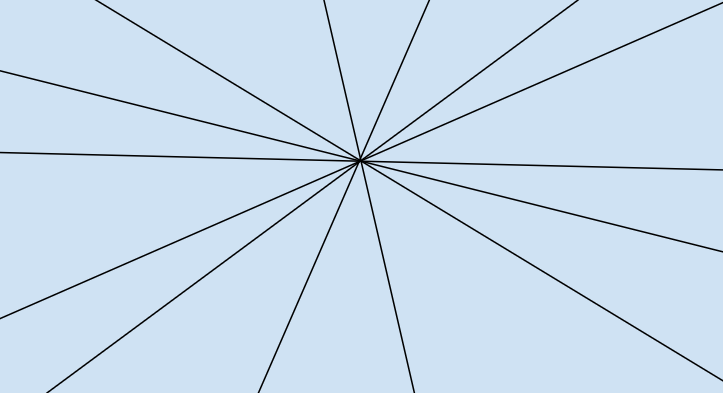
\includegraphics[width = 0.5\linewidth]{images/epipolarlines-a.PNG}
\begin{tcolorbox}[colback=white!5!white,colframe=green!75!black]
\setbox0=\hbox{\parbox[t]{\textwidth}{
    %%%%%%% ANSWER STARTS HERE %%%%%%%%%%%%%%%%%%%%%%%%%%%%

    TODO: Your answer to (a) here.

    %%%%%%% ANSWER ENDS HERE %%%%%%%%%%%%%%%%%%%%%%%%%%%%%%
    }}
\clipbox{0pt \dimexpr\dp0-8\baselineskip\relax{} 0in 0pt}{\copy0}
\end{tcolorbox}

\item Also draw or describe the relative positions of the two camera planes. Check slides from the lecture on stereo geometry for details of carera planes.\textbf{[1 point]}
\begin{tcolorbox}[colback=orange!5!white,colframe=orange!75!black]
Converge to a point outside of the image plane.
\end{tcolorbox}

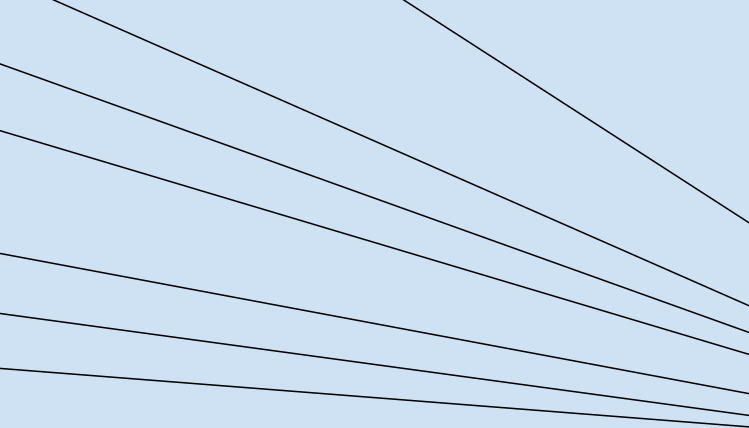
\includegraphics[width = 0.5\linewidth]{images/epipolarlines-b.PNG}

\begin{tcolorbox}[colback=white!5!white,colframe=green!75!black]
\setbox0=\hbox{\parbox[t]{\textwidth}{
    %%%%%%% ANSWER STARTS HERE %%%%%%%%%%%%%%%%%%%%%%%%%%%%

    TODO: Your answer to (b) here.

    %%%%%%% ANSWER ENDS HERE %%%%%%%%%%%%%%%%%%%%%%%%%%%%%%
    }}
\clipbox{0pt \dimexpr\dp0-8\baselineskip\relax{} 0in 0pt}{\copy0}
\end{tcolorbox}

\item \textbf{[1 point]} 
\begin{tcolorbox}[colback=orange!5!white,colframe=orange!75!black]

% OLD QUESTION:
%What might you need to change about your fundamental matrix calculations if you obtained the following epipolar lines?%

Notice the misalignment of the epipolar lines in the image below? What went wrong in the calculation of the fundamental matrix and how can we fix it?

\textit{Hint:} Check slides from the lecture on stereo geometry.
\end{tcolorbox}

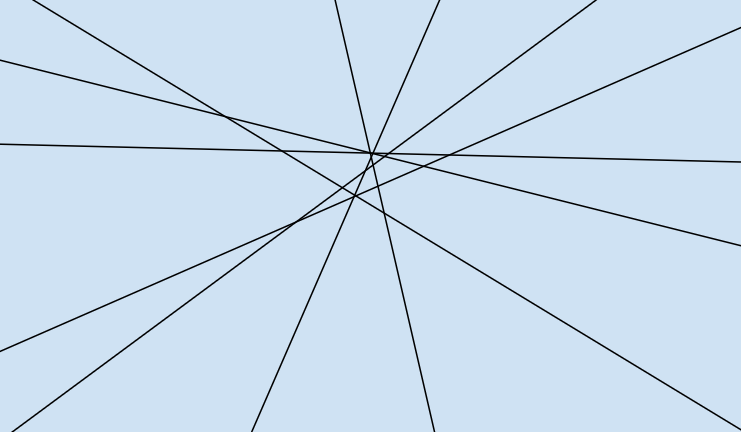
\includegraphics[width = 0.5\linewidth]{images/epipolarlines-c.PNG}
\begin{tcolorbox}[colback=white!5!white,colframe=green!75!black]
\setbox0=\hbox{\parbox[t]{\textwidth}{
    %%%%%%% ANSWER STARTS HERE %%%%%%%%%%%%%%%%%%%%%%%%%%%%

    TODO: Your answer to (c) here.

    %%%%%%% ANSWER ENDS HERE %%%%%%%%%%%%%%%%%%%%%%%%%%%%%%
    }}
\clipbox{0pt \dimexpr\dp0-8\baselineskip\relax{} 0in 0pt}{\copy0}
\end{tcolorbox}
\end{enumerate}

%%%%%%%%%%%%%%%%%%%%%%%%%%%%%%%%%%%
\pagebreak 
\paragraph{Q6a:} \textbf{[6 points]} Cameras are used in surveillance systems. One argument in favor of surveillance systems is to deter and solve crime to improve safety. Another is that if you're not doing anything wrong, you don't have anything to worry about. One argument against surveillance systems is that they compromise people's privacy even when no wrongdoing is taking place. Another is that they increase stress and anxiety.

Computer vision allows the \emph{automation} of surveillance. For instance, it lets us find the mathematical relationship between multiple cameras to track objects and people in 3D spaces, or it can reduce the burden upon a human operator who need only respond to detected events rather than actively monitor many cameras. Such functionality makes it easier to scale a surveillance operation.

On Brown's campus, the number of surveillance cameras has been increasing: compare this \href{https://www.browndailyherald.com/2008/01/10/surveillance-cameras-on-campus-triple/}{2008 Brown Daily Herald article} with this \href{https://www.browndailyherald.com/2020/02/21/cameras-installed-hegeman-hall/}{2020 Brown Daily Herald article}. While some, like those in Hegeman Hall, were installed only temporarily (\href{https://www.browndailyherald.com/article/2021/07/university-removes-hegeman-hall-surveillance-cameras}{2021 Brown Daily Herald article}), there are now 800 surveillance cameras on campus.

\begin{tcolorbox}[colback=orange!5!white,colframe=orange!75!black]
Suppose Brown both did and did not use computer vision automation. How comfortable are you with Brown's surveillance apparatus in each case?
In what circumstances do you believe that the potential benefits of surveillance \emph{automation} outweigh the potential concerns, and why? [8--10 sentences]
\end{tcolorbox}
\begin{tcolorbox}[colback=white!5!white,colframe=green!75!black]
\setbox0=\hbox{\parbox[t]{\textwidth}{
    %%%%%%% ANSWER STARTS HERE %%%%%%%%%%%%%%%%%%%%%%%%%%%%

    TODO: Your answer here.

    

    %%%%%%% ANSWER ENDS HERE %%%%%%%%%%%%%%%%%%%%%%%%%%%%%%
    }}
\clipbox{0pt \dimexpr\dp0-22\baselineskip\relax{} 0in 0pt}{\copy0}
\end{tcolorbox}


%%%%%%%%%%%%%%%%%%%%%%%%%%%%%%
\pagebreak
\paragraph{Q6b:} \textbf{[6 points]} Unmanned aerial vehicles---sometimes called drones---often carry cameras. Their cameras can be used for navigation via manually remote control, or for use within \href{https://link.springer.com/article/10.1007/s10846-017-0483-z}{sophisticated computer vision} strategies like camera pose estimation and depth estimation to enable assisted or autonomous flying in complex environments.

For your CSCI 1430 final project, you are developing a drone for \href{https://www.cnn.com/2019/05/01/health/drone-organ-transplant-bn-trnd/index.html}{life-saving organ delivery}. You create a successful computer vision algorithm that allows your drone to navigate autonomously. You are approached by several organizations that want to pay you generously for access to your project, but you are also considering open sourcing your algorithm with a permissive software license.

\begin{tcolorbox}[colback=orange!5!white,colframe=orange!75!black]
Please list three organizations that might be interested in acquiring your project for their own purposes. If each of these organizations used your project, who could benefit and how? Who could be harmed and how? Would an open-source license affect this? [6–9 sentences]
\end{tcolorbox}
\begin{tcolorbox}[colback=white!5!white,colframe=green!75!black]
\setbox0=\hbox{\parbox[t]{\textwidth}{
    %%%%%%% ANSWER STARTS HERE %%%%%%%%%%%%%%%%%%%%%%%%%%%%

    TODO: Your answer here.
    %%%%%%% ANSWER ENDS HERE %%%%%%%%%%%%%%%%%%%%%%%%%%%%%%
    }}
\clipbox{0pt \dimexpr\dp0-24\baselineskip\relax{} 0in 0pt}{\copy0}
\end{tcolorbox}


%%%%%%%%%%%%%%%%%%%%%%%%%%%%%%%%%%%
\pagebreak
\section*{Feedback? (Optional)}
We appreciate your feedback on how to improve the course. You can provide anonymous feedback through \href{https://forms.gle/Eu5jJbDUmLknAyJV9}{this form}, that can be accessed using your Brown account (your identity will not be collected). If you have urgent non-anonymous comments/questions, please email the instructor.



\end{document}
